\documentclass{uofsthesis-cs}
\usepackage{graphicx}
\graphicspath{ {images/c2/}, {images/c3/} }
\usepackage{amsmath}
\usepackage{amsfonts}
\usepackage{changes}
\definechangesauthor[name=Dave Schneider, color=red]{djs}
\definechangesauthor[name=Yujie Pei, color=green]{Yuge}
\usepackage{subcaption}

\title{An Alternative Method for Characterization and Comparison of
  Plant Root Shapes}


\author{Yujie Pei}
\degree{\MSc}
\defencedate{Month/Year}
\department{School of Environment and Sustainability}
%\Academicunit{Master of Environment and Sustainability}


%\abstract{}
%\acknowledgements{}
%\dedication{}
% LIST OF ABBREVIATIONS - Sample  
% If you don't want a list of abbreviations, comment the following 4 lines.
%\loa{\abbrev{SCUBA}{Self Contained Underwater Breathing Apparatus}
%\abbrev{LOF}{List of Figures}
%\abbrev{LOT}{List of Tables}
%}



\begin{document}

\maketitle  
%\frontmatter
\tableofcontents


\chapter{Existed Morphological Descriptors for Root Systems} % chapter 1


%__________________________ Chapter 2 _________________________________________

\chapter{An Alternatively Mathematical Method for Shape Description} 

  %__________ Section 2: heat content in annulus _______________________
  
\section{Heat Content in Annulus}

Since the heat equation, also known as the diffusion equation, defined
in an annulus possesses explicit solutions, the analytical expressions
of heat content, derived by the integration over the whole domain, are
then accessible. In this section, the preliminary step is to solve the
initial-boundary value problem (IBVP) defined in the annulus. As the
solution of IBVP and its related quantities are in the form of the
infinite series, the numerical method will be used to approximate them
to validate the research methodology in the next chapter.


\subsection{\highlight[id=Yuge, comment={Dave, Please give me the feedback or comments on this subsection.}]{Analytical Results}}\label{analytical results}

The \added[id=djs]{solution to the} $2$-dimensional heat equation \cite{crank1979mathematics}
Eq.~\ref{eq:polar_coordinate_diffusion} defined in the polar
coordinate system \added[id=djs]{, $u(r, \theta, t)$,} describes the heat distribution or temperature
varying in time and positions in the domain $\Omega$ shown in
Figure~\ref{fig:annulus} \deleted[id=djs]{. $u(r, \theta, t)$ is the unknown function to
be solved}, where $r$ is radial coordinate, $\theta$ is the angular
coordinate, $t$ is the time, $D$ is the diffusion coefficient \replaced[id=djs]{and
determines how fast $u$ changes in time}{and subscripts denote
derivatives with respect to the indicated independent variable}.

\comment[id=djs]{Use amslatex macros to improve formatting of equations and consistently use subscripts to indicate derivatives}
\begin{align}
  u_t & = D\left(u_{rr} + \frac{1}{r} u_r + \frac{1}{r^2} u_{\theta\theta}\right)
  \qquad\text{in $\Omega$}\label{eq:polar_coordinate_diffusion} \\
  u & = 0
  \qquad\text{on $\partial \Omega_1$}\label{eq:Dirichlet_bc} \\
  ru_r & = 0
  \qquad\text{on $\partial \Omega_2$}\label{eq:Neumann_bc} \\
  u(r, \theta, 0) & = \frac{1}{|\Omega|}
  \qquad\text{in $\Omega$}\label{eq:initial_bc}  
\end{align}
\added[id=djs]{Note, $|\Omega|$ is the area of the dark annulus in Fig.~\ref{fig:annulus}
  and $\partial \Omega_1$ and $\partial \Omega_2$ are disjoint subsets of the boundary of $\Omega$.}

From the microscopic and probabilistic perspective, $u(r, \theta, t)$
\comment[id=djs]{This is correct at $t=0$}{is a probability density function}, which gives the value of
\comment[id=djs]{There is no such thing as a ``heat particle''}{heat
particles at $(r,\theta, t)$\deleted[id=djs]{at time $t$}. Eq.~\ref{eq:Dirichlet_bc} and
Eq.~\ref{eq:Neumann_bc} are the homogenous Dirichlet boundary
condition and the homogenous Neumann boundary condition,
respectively. \replaced[id=djs]{In other words}{Using the heat interpretation}, the inner boundary $\partial \Omega_{1}$
is cooled to the zero temperature because the heat particles will be
absorbed when they encounter $\partial \Omega_1$. The outer boundary
$\partial \Omega_{2}$ is perfectly insulated since the heat particles
will be reflecting when they reach $\partial
\Omega_2$. Eq.~\ref{eq:initial_bc} states that the heat particles
distribute uniformly over the whole domain at \deleted[id=djs]{time} $t=0$\deleted[id=djs]{, where
$|\Omega|$ equals the total area of the annulus}.

\begin{figure}
  \centering
  
\includegraphics[width=0.5\textwidth]{annulus.png}
  \comment{I changed the caption text to show how to be more clear and comprehensive.}
  \caption{The dark annulular region, $\Omega$, is treated as a homogeneous and isotropic
    medium with relecting (Neumann) inner boundary $\partial \Omega_1$ at radius
    $a$ and absorbing (Dirichlet) outer boundary $\partial \Omega_2$ at radius
    $b$. \label{fig:annulus}}
\end{figure}

\subsubsection{Solving Heat Equation}

Generally, before solving the heat equation, it is convenient and
efficient to generate a group of dimensionless variables by
dimensional analysis. The benefit of dimensional analysis is that many
physical parameters can be combined into a smaller number of unitless
variables, which do not depend on the unit of the measurements and can
also describe the phenomenon or system of interest
\cite{barenblatt1996scaling}.


Let $\mu = b/a$ be the dimensionless radius ratio, $\tau =
\frac{Dt}{a^2}$ be the dimensionless time, and $\hat r = \frac{r}{a}$
be the unitless radius. Substitute these dimensionless variables into
Eq.~\ref{eq:polar_coordinate_diffusion} and rewrite it as

\begin{equation}\label{eq:DA_polar_diffusion}
  u_\tau = (u_{\hat r \hat r} + \frac{1}{\hat r} u_{\hat r} + \frac{1}{\hat r ^2} u_{\theta\theta})
\end{equation}

With the uniform initial condition,
\begin{equation}\label{eq:DA_initial_bc}
  u(\hat r, \theta, 0) = \frac{1}{|\Omega|}
\end{equation}

With the homogenous boundary conditions
\begin{equation}\label{eq:DA_Dirichlet_bc}
  u(1, \theta, \tau) = 0
\end{equation}

\begin{equation}\label{eq:DA_Neumann_bc}
  u'(\mu, \theta, \tau) = 0
\end{equation}



After implementing the separation of variables method
\cite{crank1979mathematics}, the solutions of
Eq.~\ref{eq:DA_polar_diffusion} with conditions
Eq.~\ref{eq:DA_initial_bc}, Eq.~\ref{eq:DA_Dirichlet_bc}, and
Eq.~\ref{eq:DA_Neumann_bc} are

\begin{equation}\label{eq:annulus_solutions_u}
  u(\hat r, \theta, \tau) = \sum_{n=1}^{\infty}
  \tilde{c_{0,n}} \bigg\{J_0(\sqrt{\lambda_{0,n}})
  Y_0(\sqrt{\lambda_{0,n}} \hat r) -
  Y_0(\sqrt{\lambda_{0,n}}) J_0(\sqrt{\lambda_{0,n}} \hat
  r)\bigg\} e^{-\lambda_{0,n}\tau}
\end{equation}

where

\begin{equation}\label{eq:coeff_u}
  \tilde{c_{0,n}} = \frac{1}{(\mu^2 - 1)}
\frac{1}{\bigg[\frac{J_0(\sqrt{\lambda_{0,n}})}{J'_0(\mu
      \sqrt{\lambda_{0,n}})}\bigg]^2 -1}
\end{equation}


Eigenvalues $\lambda_{0, n}$ $(n \in \mathbb{N}_{+})$ appeared in
Eq.~\ref{eq:annulus_solutions_u} and Eq.~\ref{eq:coeff_u} is the $n$th
positive root of the eigenfunction Eq.~\ref{eq:eigenfunction}, which
is a cross-product of the Bessel function \cite{watson1995treatise}

\begin{equation}\label{eq:eigenfunction}
  F_0(\lambda) = J_0(\sqrt{\lambda}) Y_0'(\sqrt{\lambda} \mu) -
  J_0'(\sqrt{\lambda} \mu) Y_0(\sqrt{\lambda})
\end{equation}


\subsubsection{Heat Content (Survival Probability)}

The amount of heat contained in $\Omega$ at the moment $\tau > 0$
defined as heat content $Q_{\Omega}(\tau)$, which is an alternative
terminology of survival probability $S(\tau)$ in some mathematical
literatures \cite{birkhoff1954note} \cite{van1994heat}
\cite{gilkey1994heat}. $S(\tau)$ is proportional to $Q_{\Omega}(\tau)$
\cite{kalinay2011survival}, which gives the probability of the
particles remain diffusing in the domain $\Omega$ at time $\tau > 0$
\cite{aalen2008survival}. Survival probability can be expressed by

\begin{equation}\label{eq:annulus_analytical_s}
  \begin{split}
    S(\tau) &= \int_{0}^{2\pi} d\theta \int_{1}^{\mu} \hat r d \hat r
    u(\hat r, \theta, \tau)\\ &= \sum_{n=1}^{\infty} \frac{4}{\mu^2 -
      1} \frac{1}{\lambda_{0,n}
      \bigg\{\bigg[\frac{J_0(\sqrt{\lambda_{0,n}})}{J'_0(\mu
          \sqrt{\lambda_{0,n}})}\bigg]^2 -1\bigg\}} e^{-\lambda_{0, n}
      \tau}
  \end{split}
\end{equation}

Eq.~\ref{eq:annulus_analytical_s} reveals some basic properties of
$S(\tau)$. Firstly, when $\tau=0$, the survival probability is $1$
since all the particles are just generated over the whole domain and
not be absorbed by $\Omega_1$. Secondly, $S(\tau)$ is a convergent
series with multiexponential decay. Thirdly, $S(\tau)$ interconnects
the overall geometric characteristics of $\Omega$. For example, the
decay rate of $S(\tau)$ in a short time heavily depends on the
geometrical features of $\Omega_1$, as only the particles inserted
close to $\Omega_1$ have the high probabilities of being
absorbed. Finally, as the lone-time limit, $S(\tau)$ is represented by
the lowest eigenvalue $\lambda_{0,1}$.


\subsubsection{Mean First-Passage Time}

The first passage phenomena play a fundamental role in stochastic
processes triggered by a first-passage event
\cite{van1992stochastic}. In this thesis, we only focus on the
stochastic evolution of $u(\hat r, \theta, \tau)$ until the
first-passage time, at which a heat particle reaches any sites of
target boundary $\Omega_1$ for the first time. Similarly, another
essential first-passage-related quantity is the first-passage
probability, which is a probability of the diffusing heat particles
hitting a specified site or a set of sites at a specified time for the
first time \cite{redner2001guide}. All the first-passage
characteristics can be expressed in terms of the first-passage
probability. For example, the survival probability of heat particles
at time $\tau$ calculated in the last subsection is

\begin{equation}\label{eq:pdf_fpt}
  f(\tau) = - \frac{\partial S(\tau)}{\partial \tau}
\end{equation}

where $f(\tau)$ is the first-passage probability to the target
boundary $\Omega_1$ at time $\tau$ regardless of particles' stop
positions. By the definition, the $n$th moment of the exit time
\cite{redner2001guide} is

\begin{equation}\label{eq:nth_fpt}
  \begin{split}
    \langle \tau^n \rangle &= \int_{0}^{\infty} \tau^n f(\tau) d\tau \\
    &= - \int_{0}^{\infty} \tau^n  \frac{\partial S(\tau)}{\partial \tau} d\tau \\
    &= -\tau^n S(\tau) |_{0}^{\infty} + n\int_{0}^{\infty} \tau^{n-1}S(\tau) d\tau
\end{split}
\end{equation}


Substitue $n=1$ in Eq.~\ref{eq:nth_fpt}, the mean-first passage time
$\langle \tau \rangle$, also called the average first-passage time, of
heat particles implies an overall property of the system and can be
expressed as

\begin{equation}\label{eq:mfpt}
  \begin{split}
    \langle \tau \rangle &= \int_{0}^{\infty} \tau dS\\
    &=\sum_{n=1}^{\infty} \frac{4}{\mu^2 - 1}
    \frac{1}{\lambda^2_{0,n}\bigg\{\bigg[\frac{J_0(\sqrt{\lambda_{0,n}})}{J'_0(\mu\sqrt{\lambda_{0,n}})}\bigg]^2
      -1\bigg\}}
  \end{split}
\end{equation}

 % subsection 1
  %
\newpage

\subsection{Numerical Analysis}

Numerical analysis is an area of mathematics and computer science that
creates, analyzes, and implements algorithms for approximating
numerical solutions to problems involving continuous variables
\cite{brezinski2012numerical}. For simplicity, a specific kind of
annulus is considered, which has the radius ratio $\mu=2$. 

The preliminary step of the evaluation of $S(\tau)$, a general
Dirichlet series, and $\langle \tau \rangle$ is to compute the
monotonically increasing $\lambda_{0,n}$ of Eq.$(2.7)$. The $n$th
positive zero $\lambda_{0,n}$, as $n \rightarrow \infty $, can be
bracketed in an interval $((n-1) \pi, (n+1) \pi)$
\cite{NIST:DLMF}. Bisection method \cite{2020SciPy-NMeth}, a
well-known and most reliable root finding method. It can be used to
close in on the root by successivly halving the interval until it
becomes sufficiently small.

\begin{figure}[h!]
  \centering
  \subfloat[]{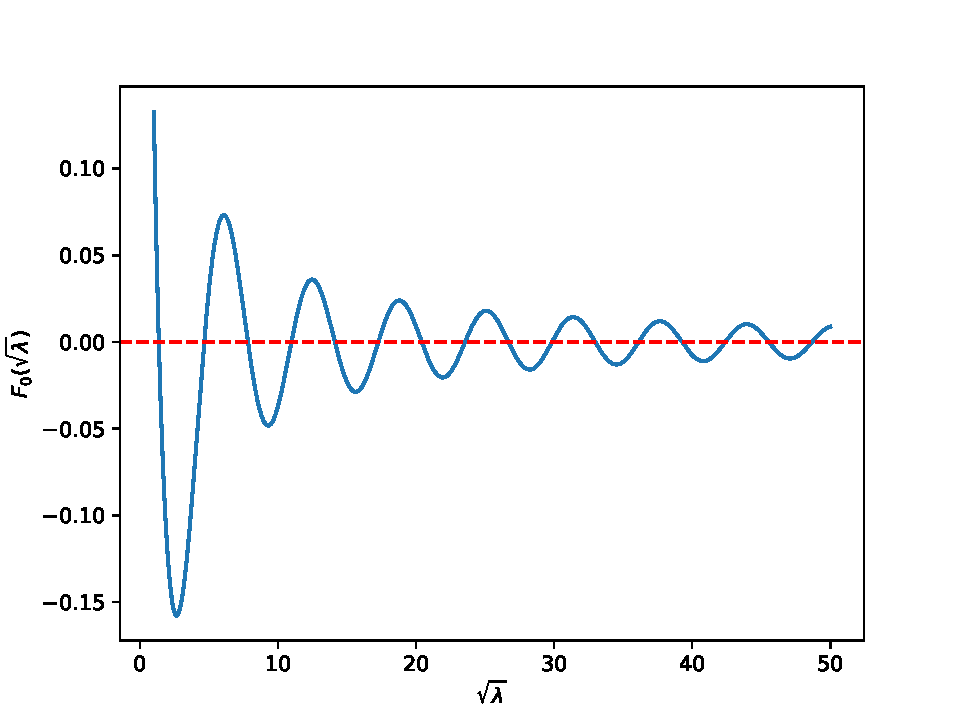
\includegraphics[width=0.5\textwidth]{F0}}%
  %\qquad
  \subfloat[]{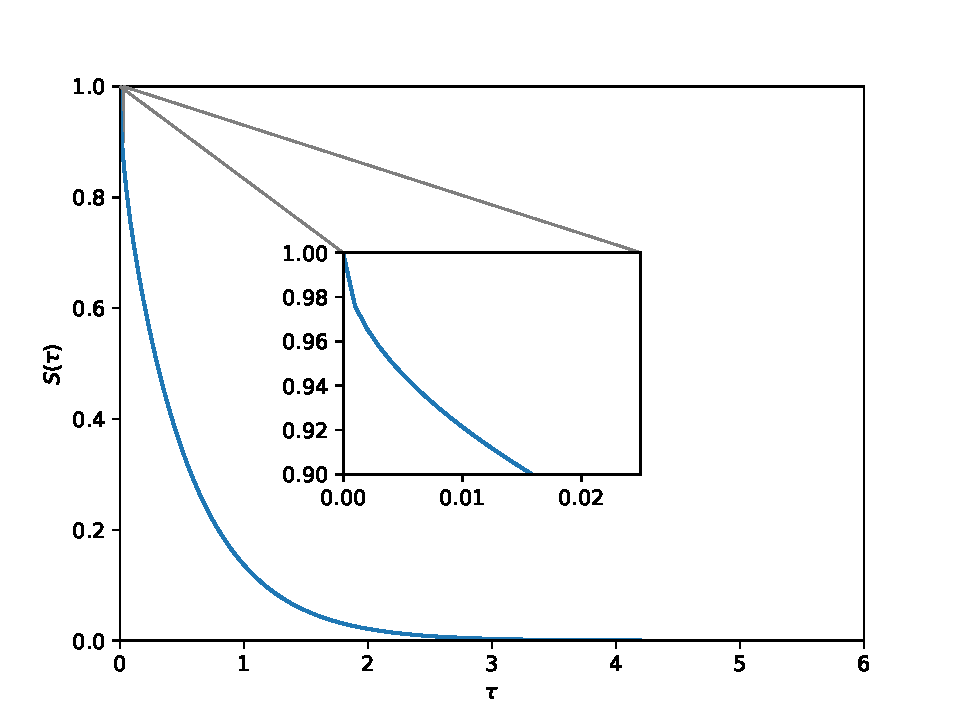
\includegraphics[width=0.5\textwidth]{analytical_s}}%
  \caption{(a) It is straightforward to evaluate the cross-product of
    Bessel fucntions by SciPy library \cite{2020SciPy-NMeth}. (b) The
    asymptotic behaviors of survival probability $S(\tau)$ are
    approximated by the numerical method with the first $1000$
    eigenvalues. $S(\tau)$ monotonously descrese from 1 at $\tau=0$ to
    $0$ as $\tau$ goes to infinity. Moreover, the approximation of
    analytical mean first-passage time $\langle \tau \rangle$ equals
    $0.47339248$.}
\end{figure}




 % subsection 2
  % ________ Section 3: Monte Carlo Simulations ________________________
  %\section{Monte Carlo Simulations}

In this section, several widely used numerical methods for solving
partial differential equations (PDEs), such as the diffusion equation,
and their limitations in practice are introduced. From the
deterministic perspective, one of the probabilistic algorithms,
Monte-Carlo (CM) methods, is proposed. However, discretization errors
also affect the accuracy of the solutions. Finally, based on the
theories of two random walk models, Pearson's random walks (PRWs) and
lattice random walks (LRWs), two fixed-time step Monte Carlo
simulations are designed. Those simulations can approximate the
integration of the heat equations' solutions, named survival
functions, which describes the geometrical properties of the shape.


\subsection{Background}

In the last section in this chapter, the exact analytical solutions of
the heat equation defined in the annulus with the initial and boundary
conditions have been derived. And then, the analytical survival
probability can be calculated by the integration over the annulus for
shape characterization. This analytical method looks useful, but its
applications to practical problems will present difficulties. Firstly,
the numerical evaluation of the analytical solutions is usually by no
means trivial because they are in the form of infinite
series. Secondly, either irregular geometries or discontinuities cause
the complication in solving the heat (diffusion) equations by
analytical methods in practice, so the explicit algebraic solutions
are close to non-existed. In other words, the analytical techniques
and solutions have a severe limitation that they can apply strictly
only to the linear form of the diffusion equations and the boundary
conditions \cite{crank1979mathematics}. Therefore, numerical methods
and computer simulations are more useful and accessible in solving
differential equations than calculating pure analytical solutions.

\subsubsection{Deterministic Numerical Methods}

The techniques for solving initial-boundary value problems (IBVPs)
based on numerical approximations have existed for a long time. The
finite-difference methods (FDM) are frequently used and easily
implemented in solving the differential equations by converting them
into a system of algebraically solvable equations
\cite{grossmann2007numerical}. The basic idea is to replace the
derivatives in the equations by difference quotients. For example, the
FTCS (Forward Time Centered Space) scheme
\cite{pletcher2012computational} aims to approximate the numerical
solutions of the heat equation and other similar parabolic PDEs. FTCS
discretizes the Laplace operator in space and the time derivative and
implements boundary conditions on the staggered grid to represent the
original continuous problem, but it is numerically stable if and only
if it satisfies a specified condition
\cite{pletcher2012computational}. Generally, there are two classes of
errors appearing in FDM called round-off error and truncation
error. The former one results from the loss of precision due to the
computer rounding of decimal quantities. The latter one is caused by
discarding the remainders in the difference approximation and highly
depends on the time and space step. In other words, the smaller the
step size, the longer the simulation duration and higher data quality
\cite{hoffman2018numerical}.


Compared with FDM, the finite element method (FEM) is particularly
solving PDEs with relatively higher quality when the problems are
defined in two or three space dimensions. FEM divides the physical
system's complicated geometries and boundaries into a certain amount
of smaller and simpler subdomains \cite{logan2011first} (eg. lattice,
triangle, curvilinear polygons, etc.). Every subdomain is locally
approximated by a finite set of element equations (piecewise shape
functions) assembled into a larger system of equations for modelling
the entire problem finally \cite{logan2011first}. The goal of FEM is
to approximate a stable solution by minimizing the associated error
function with the variational calculus \cite{logan2011first}. The
significant advantages of FEM are representing the complex geometries
accurately, exploring the local characters of the approximation, and
expressing the solutions in a unified formulation
\cite{reddy1993introduction}. However, FEM needs an amount of
mathematical skill that requires human involvement, such as converting
the original equation into the equivalent weak formulation, choosing
and changing the variational formulation and discretization strategy
in a particular problem, etc. In this thesis, the heat equations
defined in $2$-dimensional images with millions of pixels, the
extremely complex root systems and various boundary conditions, which
makes it time-consuming and challenging to trace and identify the
problems' geometries, label the nodes, and generate the coordinates
and connectivities among the nodes in the preprocessing stage of FEM.


In contrast, the finite volume method (FVM) converts the
$2$-dimensional diffusion equations into a linear equations system,
which can be solved by the direct method
\cite{eymard2000finite}. However, the accuracy of FVM is related to
the integration with respect to time and space. Unlike the domain-type
methods (e.g. FDM, FEM, FVM, etc.), the boundary element method (BEM)
is an alternative numerical computational technique for solving PDEs
formulated as an integral equation based on the boundary. Especially,
when the domain extends to infinity or the boundary is complex, BEM is
more efficient in computation than other methods because of the
smaller surface or volume ratio \cite{katsikadelis2002boundary} since
it only discretizes the boundary and fits the boundary values into the
integral equation \cite{ang2007beginner}.


However, all of the mentioned numerical methods have an intrinsically
similar feature - mesh discretization in the time and space
dimension. They need to deal with the problem in defining the
extremely complicated boundary of the root systems. If the mesh
becomes finer and the internal points number becomes larger, the
solutions of the discretized problem will converge to the original
IBVPs with a higher level of accuracy, but the computational time will
be longer. Furthermore, after applying the numerical methods, it will
sometimes take a much longer time to decide whether the solution is
right and adjust the schemes by understanding the systems
qualitatively. More importantly, the extra efforts are demanded based
on the approximated solutions of heat equations since the aimed
numerical approximation is the survival function.



%%%%%_____________________________________________________________%%%%%

\subsubsection{\textcolor{red}{\textbf{\hl{Monte Carlo Techniques}}}}


Monte Carlo (MC) methods, commonly used computational techniques, aim
to generate samples from a given probability distribution, estimate
the functions' expectations under this distribution, and optimize the
complicated objective functions by using random numbers
\cite{kroese2014monte}. Compare with the deterministic numerical
methods, applying Monte Carlo methods for solving PDEs is grid-free on
the domain, boundary, and the boundary conditions of the problem
\cite{grebenkov2014efficient}. Moreover, as the dimension of the
problem increase, those methods often become computationally expensive
while Monte Carlo methods can still provide with reasonably good
estimate at a fixed computational cost. 

Monte Carlo methods has been applied in solving $1$-dimensional and
$2$-dimensional time-dependent heat equation. The drawback of this
method is that we can only calculate the solution at one point at a
time. 

From the deterministic perspective, sloving PDEs by Monte Carlo
procedure is based on the classical probabilistic representations,
e.g. Feynman-Kac representations \cite{kac1987enigmas}, in the form of
Wiener or diffusion path integral \cite{sabelfeld2013random}. For
example, when solving the $d$-dimensional heat equation, the Brownian
motion generated by the second-order differential operator is
simulated using the numerical methods for solving the stochastic
differential equation \cite{wiki:MCMheat}. However, the discretization
step should be small enough to achieve the desired accuracy, which
will result in the long simulation.

Another straightforward approach for solving PDEs by Monte Carlo
method based on the probabilistic interpretation of integral equations
equivalent to the original continuous problem, whose solutions can be
represented as expectation of some functions of the trajectories of a
stochastic process
\cite{varadhan1980lectures}\cite{grebenkov2014efficient}\cite{sabelfeld2013random}.
Those trajectories generated by Monte Carlo techniques approximate the
expectations and the solutions. For instance, the Markov process is
proposed for estimating the expectations by simulating the successive
positions of the trajectory of the process at fixed instants with step
$\triangle t$ \cite{kronberg1976solution}\cite{king1951monte}.

%%%%%_____________________________________________________________%%%%%


\subsection{Models for Continious Diffuison Process}

Models, based on the reasoning with the averaged physical quantities,
usually lead to a diffusion equation, including concentration,
temperature, and velocity. These quantities at a space-time point
represent averages around the point in a small time interval and
spatial volume. Compared to modelling experimental and practical
situations using diffusion equations and solutions, random walk is
an entirely distinct and simplified kind of modelling procedure. It
simulates the underlying physical processes that involve the
complicated microscopic movement of atoms and molecules, in a simple
and computationally efficient way. Moreover, when averaged, the random
walk generates models that are mathematically equivalent to heat
(diffusion) equations.

\subsubsection{Borwnian Motion and Random Walks}

The heat equation describes the temperature distribution of a certain
homogeneous and isotropic domain that does not exist any heat sources
\cite{varadhan1980lectures}. In the domain, the heat spreads randomly
in all directions at some rate, so it is easier to understand
diffusion (heat) equations by considering the heat as the individual
random particle \cite{lawler2010random}. The spreading of the heat
'particles' is a diffusion process defined in continuous time with a
continuous state space and continuous sample paths
\cite{ito2012diffusion}. Brownian motion
\cite{brown1828microscopical}, also called the Wiener process, is a
case of a diffusion process with the Markov properties: future states
depend only on the present states \cite{bharucha2012elements}. From a
probabilistic perspective, the probability density of Brownian
particles satisfies the heat (diffusion) equation
\cite{kac1947random}\cite{varadhan1980lectures}.



Brownian motion \cite{brown1828microscopical}, the irregular motion of
individual pollen particles, has been existed for a long time before
the random-walk theory. At the beginning of the twentieth century, the
term, random walk, was initially proposed by Karl Pearson
\cite{pearson1905problem}. He described a simple example of the
isotropic planar random flights to model how mosquitoes migrate and
invade randomly in the cleared jungle regions. At each time step, the
mosquito moves to a random direction with a fixed step
length. Rayleigh \cite{rayleigh1905problem} stated that Pearson's
question, the distributions of mosquitos after many steps have been
taken, is the same as superpositioning the sound vibrations with unit
amplitude and arbitrary phase \cite{de2012flying}.


At almost the same time, Louis Bachelier \cite{bachelier1900theorie}
developed a model of the financial time series based on the random
walk and explored the connection between discrete random walks and
continuous diffusion (heat) equation. During the development of random
walk theory, many important fields, such as random processes, random
noise, spectral analysis, and stochastic equations, were developed by
some physicists \cite{einstein1905electrodynamics}
\cite{einstein1906theory} \cite{smoluchowski1916drei}. The continuous
Brownian motion can be considered as the limit of discrete random walk
as the time and space increments go to zero \cite{lawler2010random}.





\subsubsection{Theory of Lattice Random Walks (LRWs)}

Let us consider the heat particles perform the simple random walk on
the $d$-dimensional integer grid $\mathbb{Z}^d$. It is a
discrete-space and discrete-time symmetric hopping process
\cite{redner2001guide} on the lattice. At each time step, a random
walker moves to one of its $2d$ nearest neighbours with probability
$\frac{1}{2d}$. If $d \leq 2$, the random walk is recurrent, in which
the particle will returns to its origin infinitely often with the
probability $1$. If $d \geq 3$, the random walk is transient in which
the particle will return to its origin only finitely often with
probability $1$ \cite{hughes1998random}.


For simplicity, we start from considering $2$-dimensional lattice
random walks (LRWs) \cite{lawler2010random}. Let $\triangle l$ be the
distance between two sites and $\delta$ be the time step. Define $p(x,
t| x_{S})$ as the conditional probability of a particle to be in
position $x$ at time $t$ starting from $x_{S}$ at time $t=0$. The
temperature at a site is given by the amonunt of heat going in from
nerighboring site. Thus, $p(x, t + \delta |x_{S})$ is defined as
probability of a particle to be in position $x$ at time $t + \delta$
starting from $x_{S}$ at time $t=0$,

\begin{equation}
  p(x, t + \delta | x_{S}) = \frac{p(x - \triangle l e_{x}, t| x_{S}) +
    p(x + \triangle l e_{x}, t| x_{S}) + p(x - \triangle l e_{y}, t|
    x_{S}) + p(x + \triangle l e_{y}, t| x_{S})}{4}
\end{equation}

where $e_x$ and $e_y$ are unit vectors of $x-$ axis and $y-$ axis, respectively. 


When $\delta \rightarrow 0$, $\triangle l \rightarrow 0$, and $\delta \sim (\triangle l)^2$, 

\begin{equation}
  p(x, t | x_{S}) + \delta p(x, t | x_{S}) = p(x, t | x_{S}) +
  \frac{(\triangle l)^2}{4} (\frac{\partial ^2 p(x, t|
    x_{S})}{\partial x^2} + \frac{\partial^2 p (x, t| x_{S})}{\partial
    y^2})
\end{equation}

Finally, the $2$-dimensional heat equation is

\begin{equation}
  \frac{\partial p(x, t| x_{S})}{\partial t} = \frac{(\triangle
    l)^2}{4 \delta} (\frac{\partial ^2 p(x, t| x_{S})}{\partial x^2} +
  \frac{\partial^2 p (x, t| x_{S})}{\partial y^2})
\end{equation}
where $D = \frac{(\triangle l)^2}{4 \delta}$ is the diffusion
coefficent. This derivation shows a tight relationship between
lattice random walks and diffusion.


\subsubsection{Theory of Pearson's Random Walks (PRWs)}

Based on Pearson's problem and Rayleigh's answer, Stadje
\cite{stadje1987exact} and Masoliver et al. \cite{masoliver1993some}
considered a two-dimensional continuous-time and continuous-space
random walk, defined as Pearson's random walks (PRWs) in this thesis,
moving with constant speed and with random directions distributed
uniformly in $[0, 2\pi)$. Moreover, in PRWs, the lengths of the
  straight-line paths and the turn angles are stochastically
  independent. If the mean step length approaches zero and the time is
  big enough, the behaviours of particles in PRWs weakly converges to
  the Wiener Process \cite{stadje1987exact}, which satisfies the
  traditional heat equation.
  
  
\subsection{Output Analysis}

\subsubsection{Relationship between $t$ and $\tau$}

Particles' average one-step displacement $\triangle l$ in the
fixed-time step Monte Carlo simulations, LRWs and PRWs, are associated
with the time step is $\delta$:

\begin{equation}
  \triangle l = 2 \sqrt{D \delta}
\end{equation}
where $D$ is the diffusion coefficent.

Eq.$(2.15)$ implies that the time step $\delta$ must be designed small
enough to make sure that $\triangle l$ is shorter than the smallest
geometrical features of the boundaries. Thus, $\triangle l$ should
equal or be less than one-pixel size in the simulations. Furthermore,
the $\delta$ is regarded as a fundamental bridge between particles'
number of steps $t$ and unitless continuous-time $\tau$,

\begin{equation}
 \tau = t \delta = \frac{(\triangle l)^2 t}{4D}
\end{equation}
where $D$ is 1.

When running the LRWs in the annulus, $\triangle l$ is always
$\frac{1}{100}$ since particle's step length is as same as one-pixel
size. However, $\triangle l$ is related to the particle's step length
in PRWs. If particle's step length is $0.5$, a half of a pixel, then
$\triangle l$ equals $\frac{1}{100} \times \frac{1}{2} =
\frac{1}{200}$.  Similiarly, when the step length in PRWs is $0.1$,
then $\triangle l$ is $\frac{1}{1000}$. 


\subsubsection{Kaplan-Meier Estimator}

The general definition of the survival time is the time starting from
a specified point to the occurrence of a given event
\cite{bewick2004statistics}, such as death, pregnancy, job loss,
etc. Also, the analysis of the group of survival data is called
survival analysis \cite{altman1990practical}. In the survival
analysis, three kinds of situations will affect the subjects' survival
time \cite{goel2010understanding}. Firstly, the subjects are
uncooperative and refused to continue to participate in the
research. Secondly, some subjects do not experience the event before
the end of the study, but they would have experienced the event if
they keep being observed. Finally, the researchers lose touch with the
subjects in the middle of the investigation. In practice, since these
subjects have partial information about survival, the scientists will
label the above circumstances as censored observations
\cite{bewick2004statistics} instead of ignoring them and decreasing
sample size. 

In clinical trials or community trials, Kaplan-Meier Estimator
\cite{kaplan1958nonparametric}, a non-parametric analysis, is a
commonly applied statistical method in the survival analysis for the
measurement of the fraction of the survival time after the treatment
\cite{aalen2008survival} and for generating the corresponding survival
curve. It also works well with the mentioned three difficult
situations. With various assumptions \cite{etikan2017kaplan}
\cite{goel2010understanding}, the Kaplan-Meier survival curve can be
created and provides the probability of surviving in a given length of
time while considering the time in many small intervals
\cite{altman1990practical}.


The output of random walk models is particles' wandering time, also
defined as the number of steps, before encountering the absorbing
boundary. Particle's behaviours are affected by the boundary
conditions, and each of them carries some partial geometrical
information of the edges. In this thesis, the numerical survival
functions, which can be estimated by \cite{aalen2008survival}

\begin{equation}
  \widehat{S}(t) = \prod_{i:t_i \leq t} (1 - \frac{d_i}{n_i})
\end{equation}

where $t_i$ is a time when at least one particle reaches the absorbing
boundary, $d_i$ the number of particles encountering with the target
boundary at time $t_i$, and $n_i$ is the number of particles which
have not yet stopped moving up to time $t_i$.


\subsection{Sample Size Determination}

Based on the law of large number (LLN) \cite{dekking2005modern}, as
the sample size approaches infinity, the sample mean tends to get
closer to the true population mean with the high
probability. Moreover, the central limit theorem (CLT)
\cite{dekking2005modern} illustrates how the sampling distribution of
the mean changes as a function of the sample size and how much more
reliable a large experiment is. On the downside, the increasing number
of trials results in the higher cost of performing the simulation,
which is the major drawback of the fixed time-step Monte Carlo
simulations. Therefore, it is necessary to conduct the minimum number
of simulation runs to achieve a desired degree of precision.


\subsubsection{General Method}

There are five parts of the standard way to determine the sample size
in the Monte Carlo simulations. Firstly, simulating with a certain
amount of samples. Secondly, repeating the simulation several times
with the sample size as the same as the first step.  Thirdly,
increasing the number of samples and implementing the first two steps
again. Fourthly, running a regression analysis of the variability of
the sample statistic as a function of sample size. Finally, estimating
the sample size that will result in any desired level of convergence
by some probabilistic inequalities, including Chebyshev's inequality
\cite{chebyshev1867valeurs}, Cantelli’s inequality
\cite{cantelli1929sui}, Vysochanskij–Petunin inequality
\cite{vysochanskij1980justification}, etc.


\subsubsection{Dvoretzky–Kiefer–Wolfowitz (DKW) inequality}

Although the sample size estimated by the general method does not
depend on the geometries characterized by the random walk models, how
long the simulation will run is unknown, and the final calculated
sample size will be larger than the really necessary value
sometimes. Therefore, an alternative method, named the
Dvoretzky–Kiefer–Wolfowitz (DKW) inequality
\cite{dvoretzky1956asymptotic}, is proposed for the sample size
determination without simulating random walk models and considering
the shape of objects in the images.

Let $F_N(x)$ denote the empirical distribution functions (empirical
CDF) for a sample of $N$ real-valued $i.i.d.$ random variables,
$X_{1}, ... , X_{N}$, with continuous cumulative distrbution function
(CDF) $F(x)$. The DKW inequality, as expressed in Eq.$(2.18)$, bounds the
probability that the random function $F_{N}(x)$ differs from the true
$F(x)$ by more than a given constant $\varepsilon$
\cite{dvoretzky1956asymptotic}.

\begin{equation}
  Pr(\sup_{x \in \mathbb{R}} |F_{N}(x) - F(x)| > \varepsilon) \leq
  2e^{-2N\varepsilon^2} \;\; \;\; for \; every \; \varepsilon > 0
\end{equation}

The equally spaced confidence bounds or simultaneous band around the
$F_{N}$ encompassing the entire $F(x)$ can be expressed by
\begin{equation}
  F_{N}(x) - \varepsilon \leq F(x) \leq F_N(x) + \varepsilon \; \; \; \; 
\end{equation}

On the other hand, assume the simultaneous band produced by Eq.$(2.19)$
containing the $F(x)$ at a given confidence level $1-\alpha$, the
interval $\varepsilon$ can be calculated by

\begin{equation}
  \varepsilon = \sqrt{\frac{\ln{\frac{2}{\alpha}}}{2N}}
\end{equation}


Given a converge probability $\alpha$ and constant $\varepsilon$, it is
straightforward to estimate the sample size $N$ in the fixed-time step
Monte Carlo simulations in any images by Eq.$(2.20)$.


  % ________ Section 4: Two-Sample Statistical Tests ___________________
  %\section{Two-sample Statistical Tests}\label{statistical tests}

The differences between the survival curves generated by the
Kaplan-Meier estimator are visible sometimes. However, the
dissimilarities won't be easily detected by eyes if the survival
curves are overlapping over some parts or crossing at some time
points.  Since the Kaplan-Meier estimator does not provide any
information on whether two groups of survival data are statistically
similar or different, some popular statistical tests used specially in
the survival analysis course are presented in this section. Which test
should be selected in a specific circumstance is always debated
because there is a fine line between the statistical tests in the
survival analysis. Therefore, acknowledging the data in hand and
identifying the assumptions well is a prerequisite to determine the
tests appropriately.

Before listing the pros and cons of several statistical tests, the
censored survival times will be recalled firstly, which indicates the
time at which a subject is unobserved and the time to the event of a
subject is not recorded \cite{etikan2018choosing}. In this thesis, it
is possible to appear the censoring observation in the beginning or at
any other moment during the Monte Carlo simulations. If the simulation
finished, but the particle did not reach the target boundary, the
particle will be regarded as a right-censored. When the particle is
abandoned and not been observed during the simulations, it is termed
the random right censoring \cite{etikan2018choosing}. Another cause of
a deficient observation of particles' survival times is the left
censoring, which hints that the particles had stopped diffusing before
the simulation began. For instance, the particle is generated in or on
the pixels of roots. As mentioned in the last section, the
Kaplan-Meier method can still cope well with the right-censored and
left-censored observations in output.


In survival analysis, as the time interval gets close to $0$, the
instantaneous hazard rate can be calculated by limiting the number of
events per unit time divided by the number of events at risk
\cite{case2002interpreting}. The hazard ratio is an estimate of the
hazard rate in one group relative to that in another group
\cite{singh2011survival}. If the survival curves are parallel with the
identical shape, the hazard ratio is constant at any interval of
time. In this situation, the log-rank tests, also named the
Mantel-Haenszel, are reliable \cite{custodio2007diagnostics}.

If the hazard ratio does not satisfy the assumption, the log-rank test
will not be powerful to detect the differences in the survival
functions. In such a case, the Gehan-Breslow-Wilcoxon test, also
called Gehan’s generalized Wilcohon procedure, should be considered
alternatively \cite{agarwal2012statistics}. Also, under the constant
hazard ratio assumption, the Wilcoxon tests might be more reliable
than the log-rank tests \cite{custodio2007diagnostics}. The former one
gives more weight to the early failures, but the latter one is more
suitable for comparing the later events in the data
\cite{custodio2007diagnostics}. Generally, some general non-parametric
tests, based on the rank ordering (e.g. Mann-Whitney U test,
Kruskal-Wallis, etc.), are not always feasible in censoring survival
data \cite{agarwal2012statistics}. However, Gehan’s generalized
Wilcohon test is still robust when the censoring rates are low, and
the censoring distributions of groups are equal
\cite{karadeniz2017examining}.


Neither log-rank test nor Gehan’s generalized Wilcohon test can work
well when the survival curves cross while the Tarone-Ware test should
be chosen \cite{leton2001equivalence}. It pays more attention to the
failures happening somewhere in the middle of study
\cite{etikan2017kaplan}. Moreover, there is no limitation of the
number of groups when the Tarone-Ware test is applied
\cite{custodio2007diagnostics}. Similarly, the Fleming-Harrington test
is also accessible and robust for testing the differences between two
or more survival curves in the right-censored data based on the
counting process \cite{harrington1982class}.

















%__________________________ Chapter 3 _________________________________________
  
\chapter{Fixed-time Step Monte Carlo Simulations on Artificial Images}
  \section{Methodology Validation}

In the last chapter, the survival probability $S(\tau)$ and the mean
first-passage time has been calculated by solving the heat equation
and approximated by the numerical methods. Lattice Random Walks (LRWs)
and Pearson's Random Walks (PRWs) are implemented in the annulus
image, as shown in Figure $2.1$, in Python. This section aims to
validate the research methodology by comparing the estimated survival
functions $S(t)$ of the numerical data with the analytical solutions
$S(\tau)$ where $t$ is the number of steps taken by the particles in
the fixed-time step Monte Carlo simulations and $\tau$ denotes the
unitless time.


\subsection{Statistical Fluctuation Analysis}

Fixed-time step Monte Carlo simulations, LRWs and PRWs, are the
virtual representations of the original statistical problem defined in
the continuous-time and continuous-space with numerous inputs and
discrete-time trajectories sampled randomly over and over again, which
results in the statistical fluctuation. 

The first kind of error stems from the sampling. As shown in Figure
$3.1 (a)$, the larger sample size in the simulations, the estimated
survival functions will be more precise. LRWs are used to mimic the
continuous-time and continuous-space diffusion process by generating
the discrete random trajectories in the discrete time, which results
in the time-discretization and space-discretization errors. Although
PRWs is a model defined in continuous-time and continuous-space, the
random paths demand much longer time simulation as shown in Figure
$3.1 (b)$.

\clearpage

\begin{figure}[h!]
  \centering
  \subfloat[]{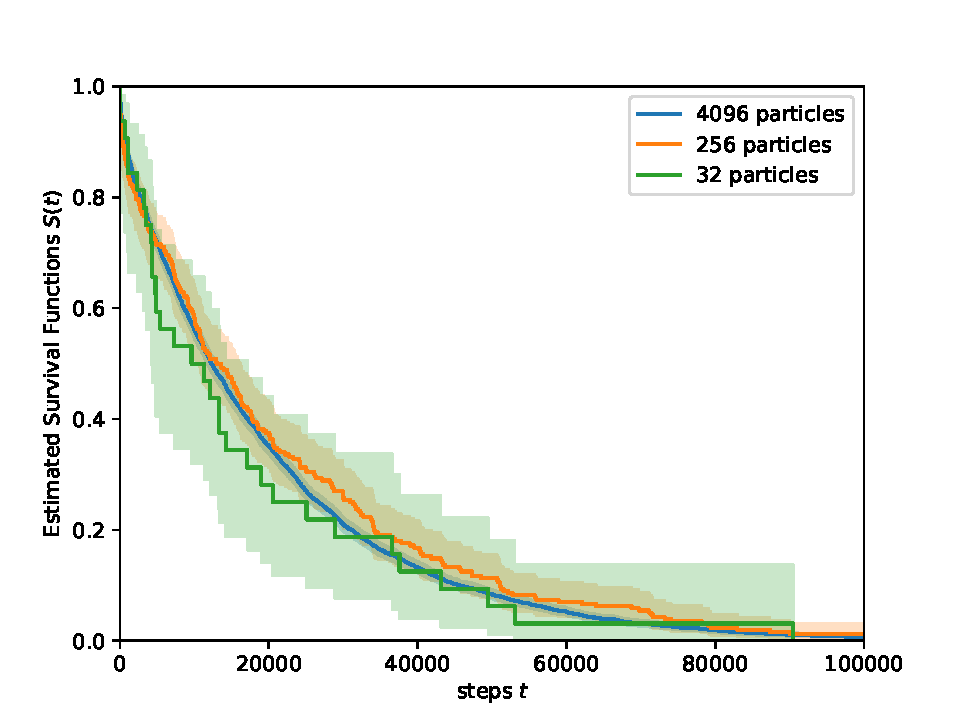
\includegraphics[width=0.5\textwidth]{sampling}}%
  %\qquad
  \subfloat[]{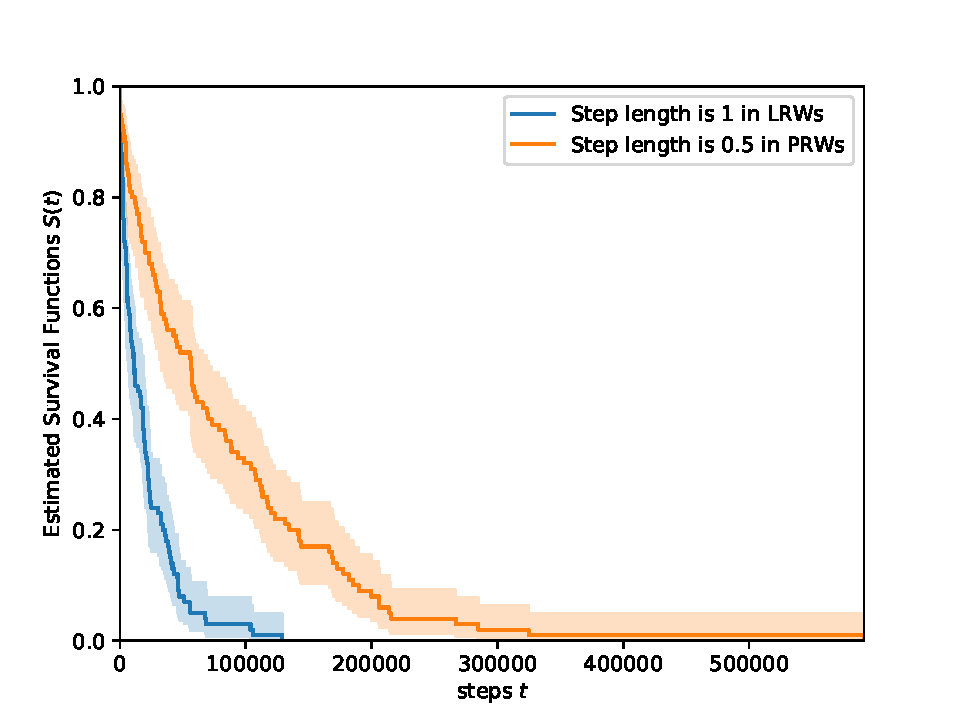
\includegraphics[width=0.5\textwidth]{discretization}}%
  \caption{(a) As the number of particles increasing, the uncertainty
    of the LRWs simulation are lower since the confidence band of the
    estimated survival function becomes narrower. (b) When run LRWs
    and PRWs in the annulus with $100$ particles, the finer
    discretization step results in the longer simulation time. }
\end{figure}


\subsection{Sample Size Determination and Evaluation}

In the last chapter, two approaches used to determine the appropriate
sample size in the fixed-time step Monte Carlo simulations have been
proposed. One of them is based on inferential statistics
\cite{casella2002statistical}, which infers and estimates the unknown
population parameters from the sample statistics. Another one is
simpler since it does not need any simulations.

\subsubsection{Chebyshev's inequality}

According to LLN \cite{dekking2005modern}, the unknown population mean
first-passage time $\bar X$ can be estimated by sample mean $\bar X_N$
when $N$ is big enough. Chebyshev’s inequality
\cite{chebyshev1867valeurs} is a probabilistic inequality that can be
applied to any probability distribution of a random variable with the
finite expected value and non-zero variance. This inequality provides
an upper bound to the probability that the absolute deviation of a
random variable from its mean will exceed a given threshold.

\clearpage


\begin{figure}[h!]
  \centering
  \subfloat[]{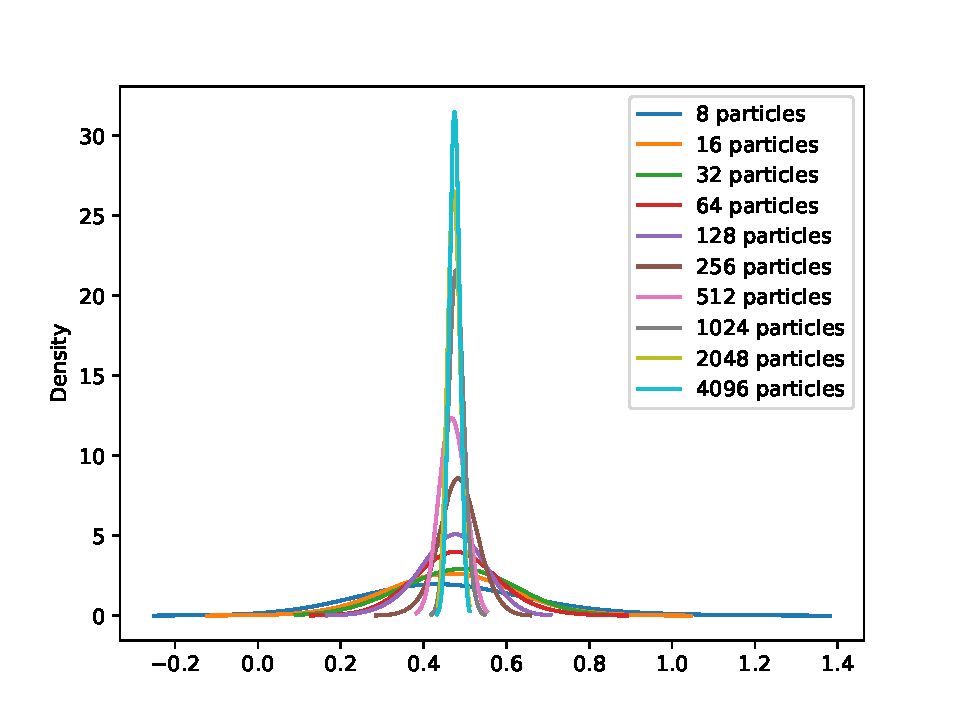
\includegraphics[width=0.5\textwidth]{kde}}%
  %\qquad
  \subfloat[]{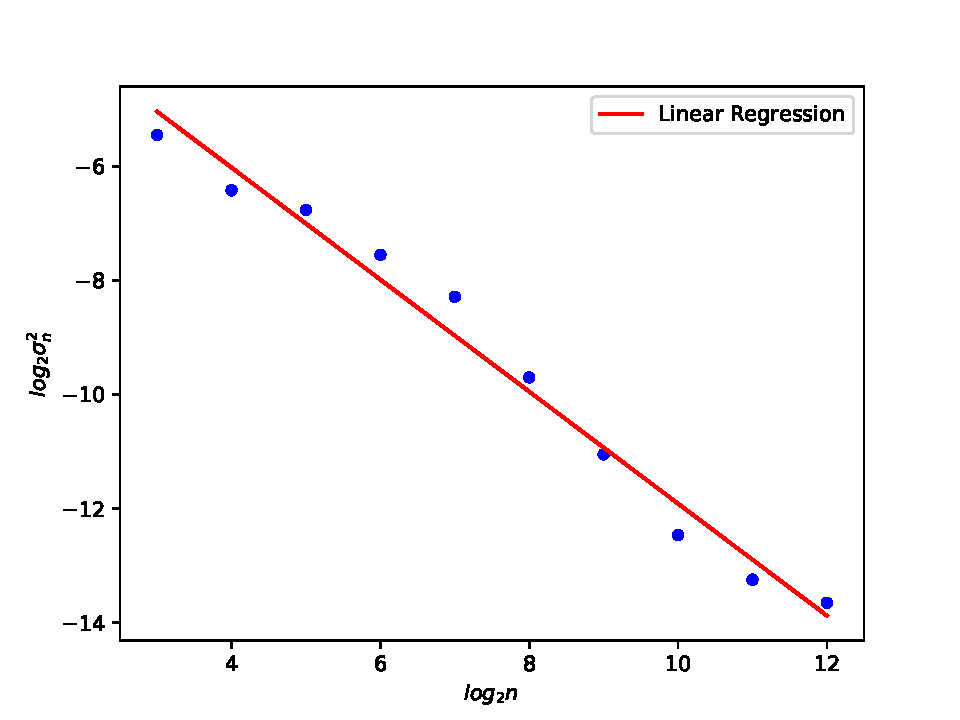
\includegraphics[width=0.5\textwidth]{linear_regression}}%
  \caption{(a) Running the LRWs in the annulus with $N = 2^i$
    particles and calculating the mean first-passage time $X_N$, where
    $i=3, 4, 5, ..., 12$. For each $N$, replicating the simulation
    $50$ times and recalculating the mean of the mean first-passage
    time $\bar X_{N}$ and the variance $\sigma^2_{N}$. As the sample
    size $N$ increase, the distribution of the sample means $X_N$
    becomes narrower and approximately normal. (b) A fitted linear
    regression model is used to explore the scaling relationship
    between $log_{2} (\sigma^2_{N})$ and $log_{2} N$. $log_{2}
    (\sigma^2_{N}) \approx b + k log_{2} N$, where $k$ and $b$ are the
    estimated model parameters, slope and intercept, respectively.}
\end{figure}

In the Figure $3.2$, the number of steps $t$ in the numerical
simulations have been converted into the unitless time $\tau$ by the
Eq.$(2.16)$. Thus, given a predesignated error $\epsilon$, the
required number of particles $N$ can be determined by

\begin{equation}
  Pr(|X_{N} - \bar X| \geq \epsilon) = Pr(|X_{N} - \bar X_{N}| \geq
  \epsilon) \leq \frac{\sigma^2_{N}}{\epsilon^2} \approx \frac{2^b
    N^k}{\epsilon^2} = 0.01
\end{equation}

where $\epsilon = 0.01 \bar X$.

The required number of particles in LRWs and PRWs can be estimated by
Eq.(3.3), which is

\begin{equation}
  N \geq (\frac{0.01 \epsilon^2}{2^b})^{\frac{1}{k}} \approx 1338643
\end{equation}

where $\epsilon \approx 0.004744$, $b \approx -2.088495$, and $k
\approx -0.982400$. Therefore, the number of particles should be at
least $1338643$ to make sure that there is no more than $1\%$ chance
of $X_N$ to be outside $[0.46865856, 0.47812641]$.


\clearpage

\begin{figure}[h!]
  \centering
  \subfloat[]{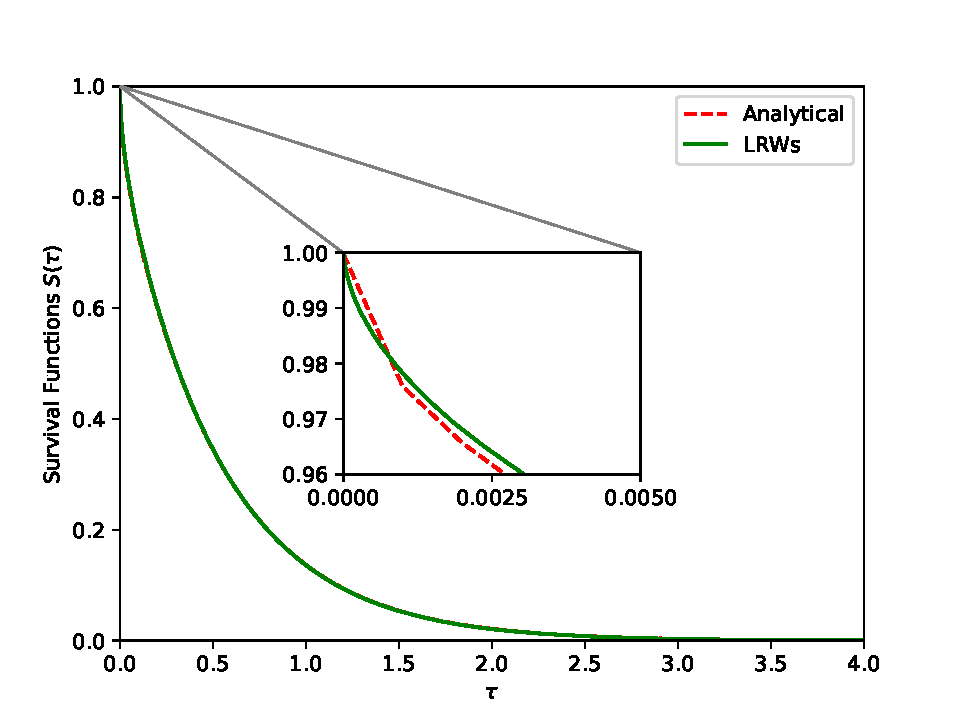
\includegraphics[width=0.8\textwidth]{LRWscheb}}%
  \qquad
  \subfloat[]{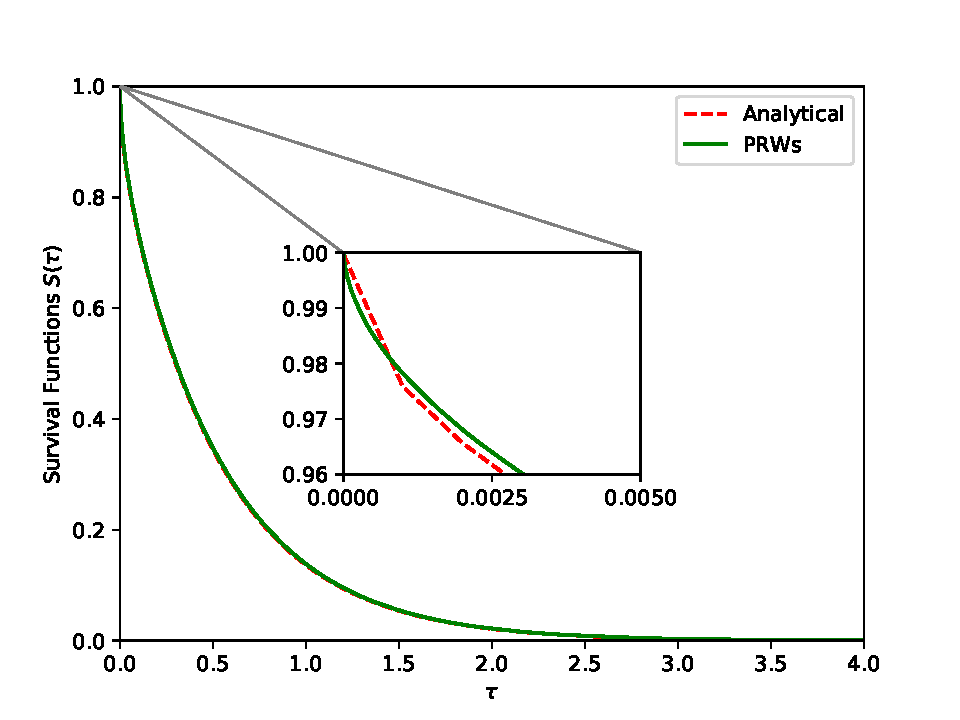
\includegraphics[width=0.8\textwidth]{PRWscheb}}%
  \caption{Running PRWs and LRWs in the annulus with $1338643$
    particles determined by the Eq.$(3.2)$.  (a) and (b) illustrate
    that the short and long time asypototic behaviors of the estimated
    survival functions of particles' diffusing times in LRWs and PRWs
    are consistent with the analytical result.}
\end{figure}

\clearpage


\begin{table}[h!]
  \centering
  \begin{tabular}{|c|c|c|}\hline
    Test Methods (standard nonparametric) & Statistics & P Values \\
    \hline
    Logrank & 0.017679 & 0.894223 \\
    \hline
    Fleming-Harrington & 0.742536 & 0.388850 \\
    \hline
    Gehan-Breslow & 0.742536 & 0.388850 \\
    \hline
    Tarone-Ware & 0.499418 & 0.479756 \\
    \hline
  \end{tabular}
  \caption{The estimated survival function of $1338643$ particles in
    the LRWs is statistically similar to the analytical survival
    function. }
\end{table}


\begin{table}[h!]
  \centering
  \begin{tabular}{|c|c|c|}\hline
    Test Methods (standard nonparametric) & Statistics & P Values \\
    \hline
    Logrank & 0.039142 & 0.843168 \\
    \hline
    Fleming-Harrington & 0.083388 & 0.772757 \\
    \hline
    Gehan-Breslow & 0.083388 & 0.772757 \\
    \hline
    Tarone-Ware & 0.010582 & 0.918069 \\
    \hline
  \end{tabular}
  \caption{The estimated survival function of PRWs, which has
    $1338643$ particles with step length $0.5$, is not statistically
    different from the analytical survival function.}
\end{table}


From the visualized comparison in Figure $3.3$ and the results of the
two-sample statistical tests, the fixed-step Monte Carlo simulations'
results converge to the analytical outcomes. Therefore, the integral
of the solutions of heat equations can be approximated by the Monte
Carlo simulations without calculating manually. As mentioned in the
last chapter, the integral, $S(\tau)$, indicates the annulus'
geometrical information. Therefore, the fixed-time step Monte Carlo
simulation can describe the shape of an object without using the
rulers. However, the number of particles in the numerical simulations
estimated by Eq.$(3.1)$ is abundant, which causes a high computational
cost because each random trajectories of each particle are simulated
in LRWs and PRWs till they reach the inner boundary of the annulus. 


\subsubsection{Dvoretzky–Kiefer–Wolfowitz (DKW) inequality}

Chebyshev's inequality can be applied to any probability distribution,
but it is also weaker than other inequalities. DKW inequality is more
efficient since the confidence band is generated without running any
simulations. For example, let $F(\tau)$ be the true cumulative
distribution function (CDF) of the first passage time, a continuous unitless
random variable on the interval $[0, \infty]$. $F(\tau)$ has a
relationship with $S(\tau)$, which is

\begin{equation}
  F(\tau) = 1 - S(\tau)
\end{equation}

The true CDF is known by Eq.$(3.3)$, which can also be approximated
numerically. A simple example of generating the CDF-based confidence
bounds by DKW inequality is shown in Fig.$3.4$. The empirical
distribution function $F_{256}(\tau)$ is estimated by the lifeline
module in Python \cite{davidson2019lifelines}. Thus, the interval
$\varepsilon$ contains the entire $F(\tau)$ with the probability
$95\%$ can be calculated by Eq.$(2.20)$

\begin{equation}
  \varepsilon = \sqrt{\frac{\ln{\frac{2}{0.05}}}{2* 256}} \approx 0.084881
\end{equation}

\begin{figure}[h!]
  \centering
  \subfloat{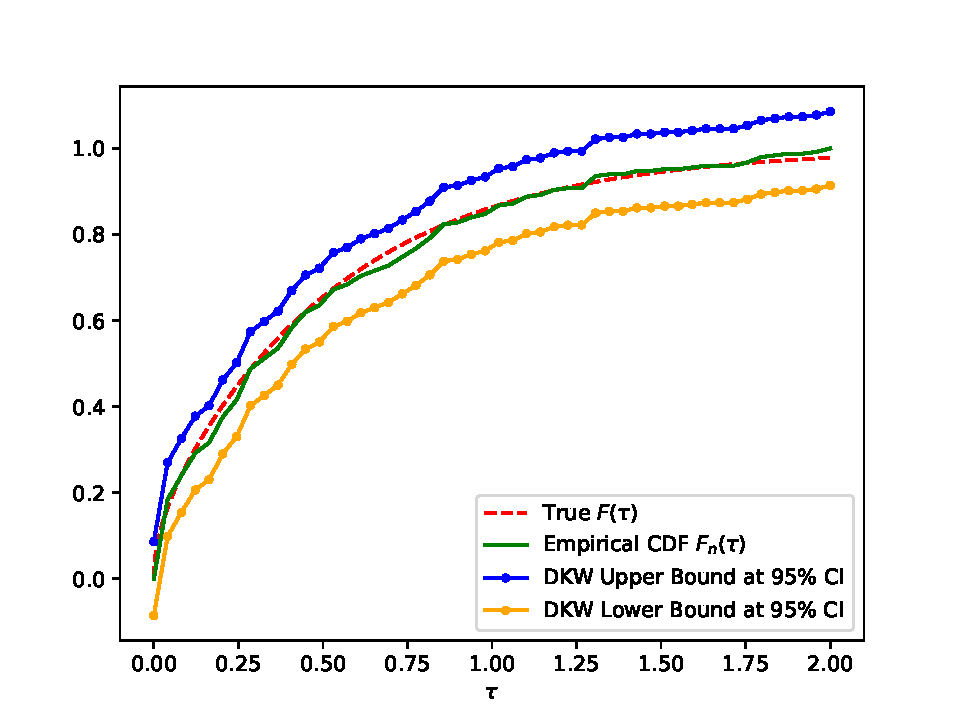
\includegraphics[width=0.8\textwidth]{dkw_comfidence_band_demo}}%
  \caption{The simultaneous band around $F_{256}(\tau)$ with interval
    $0.084881$ calculate by Eq.$(3.4)$ encompasses the entire $F(x)$
    at $95\%$ confidence level.}
\end{figure}



Moreover, the sample size estimated by DKW inequality Eq.$(2.20)$ does
not depend on the geometries or the kind of simulations because the
simultaneous confidence bounds always contain the true cumulative
distribution at a specific confidence level. For instance, assume the
probability, that the maximum distance between $F_N(\tau)$ and
$F(\tau)$ is bigger than $0.005$, is smaller than $0.01$, the minimum
required number of particles should meet the inequality

\begin{equation}
  Pr(\sup_{x \in \mathbb{R}} |F_{N}(\tau) - F(\tau)| > 0.005) \leq 2e^{-2N0.005^2} = 0.01
\end{equation}

Thus

\begin{equation}
  N \geq \frac{\ln(\frac{0.01}{2})}{-2 \times 0.005^2} \approx
  105966
\end{equation}


\clearpage

\begin{figure}[h!]
  \centering
  \subfloat[]{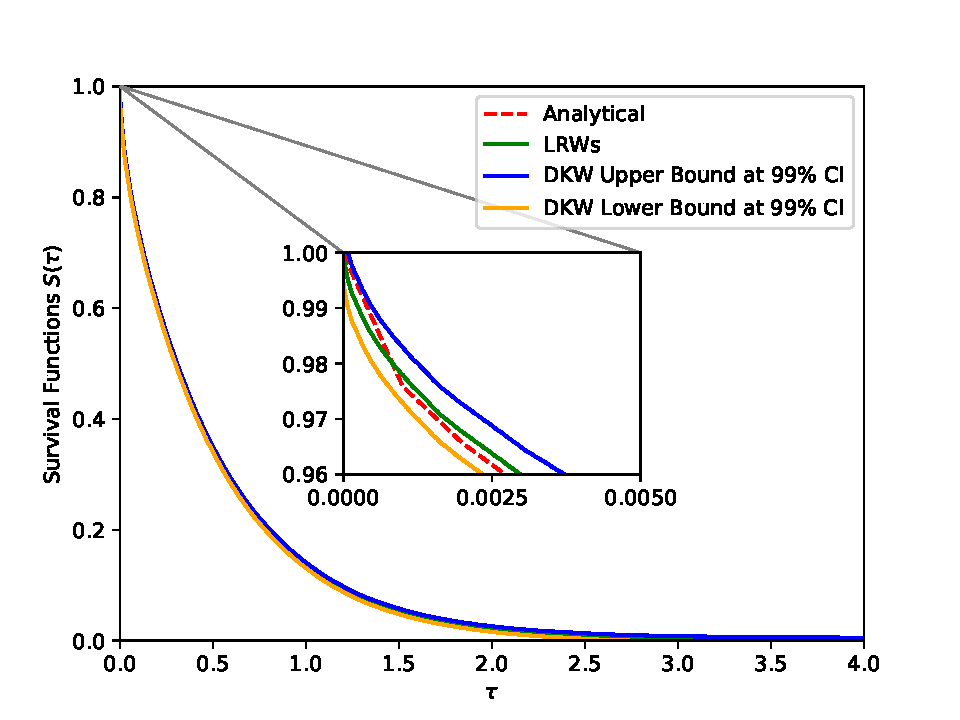
\includegraphics[width=0.8\textwidth]{LRWsdkw}}%
  \qquad
  \subfloat[]{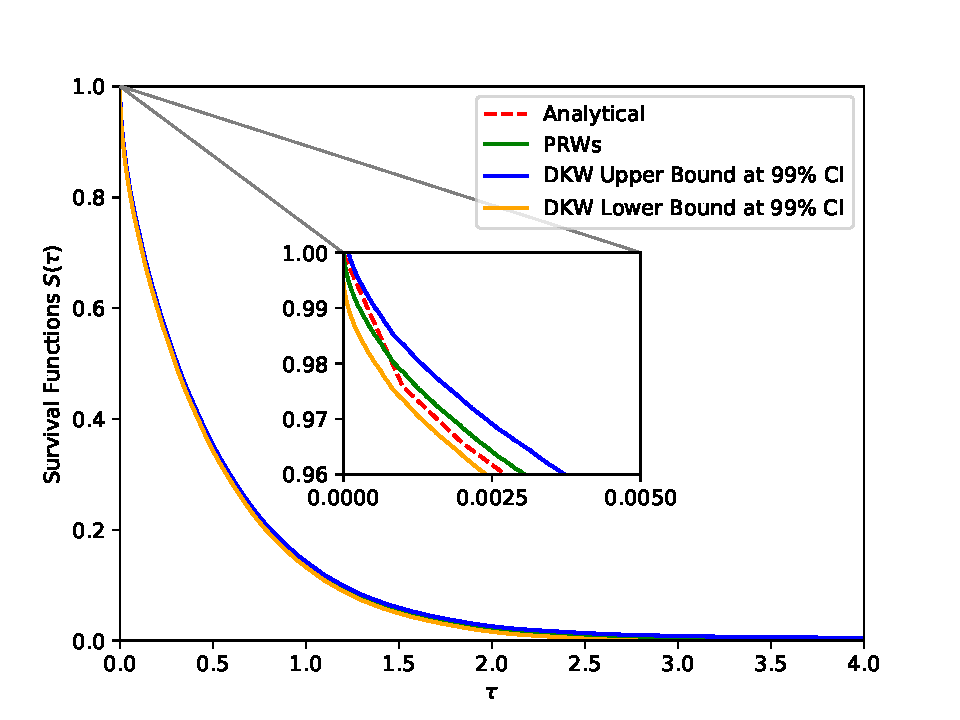
\includegraphics[width=0.8\textwidth]{PRWsdkw}}%
  \caption{PRWs and LRWs are implemented in the annulus with $105966$
    particles determined by the Eq.$(3.6)$. (a) and (b) show that the
    simultaneous confidence bands of estimated survival function with
    the interval $0.005$ contain the entire analytical $S(\tau)$ at
    $99 \%$ confidence level.}
\end{figure}

\clearpage


\begin{table}[h!]
  \centering
  \begin{tabular}{|c|c|c|}\hline
    Test Methods (standard nonparametric) & Statistics & P Values \\
    \hline
    Logrank & 1.532224 & 0.215779 \\
    \hline
    Fleming-Harrington & 1.630358 & 0.201654 \\
    \hline
    Gehan-Breslow & 1.630358 & 0.201654 \\
    \hline
    Tarone-Ware & 1.619530 & 0.203157 \\
    \hline
  \end{tabular}
  \caption{The estimated survival function of $105966$ particles in
    the LRWs is not statistically different to the analytical survival
    function. }
\end{table}


\begin{table}[h!]
  \centering
  \begin{tabular}{|c|c|c|}\hline
    Test Methods (standard nonparametric) & Statistics & P Values \\
    \hline
    Logrank & 2.645624 & 0.103835 \\
    \hline
    Fleming-Harrington & 1.473674 & 0.224767 \\
    \hline
    Gehan-Breslow & 1.473674 & 0.224767 \\
    \hline
    Tarone-Ware & 1.986810 & 0.158675 \\
    \hline
  \end{tabular}
  \caption{The estimated survival function of PRWs, which has
    $105966$ particles with step length $0.5$, is statistically
    similar to the analytical survival function.}
\end{table}


\subsection{Conclusion}


Instead of calculating the asymptotic expansion of the heat content
manually as $\tau \rightarrow 0^+$, the total heat energy $\beta$
\cite{gilkey1994heat} for time $\tau > 0$ can be approximated by the
fixed-time step Monte Carlo simulations for describing the full-scale
geometrical features of the annulus. Moreover, the required number of
particles in the simulations determined by the DKW inequality is much
smaller than the superabundant value estimated by Chebyshev’s
inequality. 










% The Bibliograpy should go here. BEFORE appendices!
\uofsbibliography{thesisref}


%%%%%%%%%%%%%%%%%%%%%%%%%%%%%%%%%%%%%%%%%%%%%%%%%%%%%%%%%%%%%%%%%%%%%%%%%
% APPENDICES
%
% Any chapters appearing after the \appendix command get numbered with
% capital letters starting with appendix 'A'.
% New chapters from here on will be called 'Appendix A', 'Appendix B'
% as opposed to 'Chapter 1', 'Chapter 2', etc.
%%%%%%%%%%%%%%%%%%%%%%%%%%%%%%%%%%%%%%%%%%%%%%%%%%%%%%%%%%%%%%%%%%%%%%%%%%

% Activate thesis appendix mode.
%\uofsappendix

% Put appendix chapters in the appendices environment so that they appear correcty
% in the table of contents.  You can use \input's here as well.

%\begin{appendices}

%\chapter{Sample Appendix}

%Stuff for this appendix goes here.

%\chapter{Another Sample Appendix}

%Stuff for this appendix goes here.

%\end{appendices}

\end{document}
